\chapter{Coupled Results}
\label{ch:coupledResults}

\section{Power Reactor Modeling}
\label{sec:power_reactor_modeling}
  The motivation for this work is to model nuclear power reactors with
  multiphysics feedback. This has been accomplished by modeling power
  distribution with the multigroup neutron diffusion equation solved via the
  Finite Element Method (FEM) (\chref{ch:neutronDiffusion}), axial heat
  convection and radial heat conduction models (\chref{ch:thermalHydraulics}),
  and simplified thermal expansion modeling (\chref{ch:thermalExpansion}).
  Combined, these effects will provide feedback which can be estimated in the
  model. 
  
  A realistic reactor benchmark is provided and modeled \sref{sec:abr}.
  Reactivity coefficients describing system responses are defined in
  \sref{sec:reactivity_coefficients}. Results are presented in
  \sref{sec:results}.

\section{Advance Burner Reactor -- MET 1000}
\label{sec:abr}
  This problem is proposed by Organisation for Economic Co-operation and
  Development Nuclear Energy Agency (OECD NEA) in \cite{abr}. The Advanced
  Burner Reactor (ABR) is fueled with a ternary metallic fuel and has a 1000
  \units{MWth} rating. This is a medium-sized metalic reactor with a total of
  180 assemblies and is 4.8 \units{m} tall. The benchmark is fully specified and
  thirty-one independent results are submitted. Each submission has generated
  its own cross-sections. Submissions include a solution using \dif.

  The materials in the benchmark are shown in \fref{fig:abr_materials}. Fast
  neutron flux is shown to peak in the core center and thermal neutron flux is
  shown to peak in the structural material surrounding the core in
  \fref{fig:abr_fluxes}.

  \begin{figure}
    \centering
    \includegraphics[width=0.4\textwidth]{abr_materials}
    \caption{Materials in ABR.}
    \label{fig:abr_materials}
  \end{figure}

  \begin{figure}
    \centering
    \subfloat[$\phi_{1}$]{
      \includegraphics[width=0.25\textwidth]{abr_phi_nod_group1}}
    \hspace{0.2in}
    \subfloat[$\phi_{33}$]{
      \includegraphics[width=0.25\textwidth]{abr_phi_nod_group33}}
    \caption{Multigroup Neutron Flux in ABR.}
    \label{fig:abr_fluxes}
  \end{figure}

\section{Reactivity Coefficients}
\label{sec:reactivity_coefficients}
  Reactivity of a reactor serves to compare the state of the reactor to the
  critical state.
  \begin{equation}
    \label{eq:reactivity}
    \rho \units{pcm} = \frac{\keff-1}{\keff} \times 10^5
  \end{equation}
  Recall $\keff < 1$ for a subcritical reactor, $\keff=1$ for a critical
  reactor, and $\keff > 1$ for a supercritical reactor. Therefore $\rho < 0$
  for a subcritical reactor, $\rho = 0$ for a critical reactor, and $\rho > 0$
  for a supercritical reactor. 

  A reactivity coefficient can be defined as a partial derivative with respect
  to a quantity of interest. Let $\alpha_x$ be the reactivity coefficient for
  quantity $x$, then
  \begin{equation}
    \label{eq:reactivity_coefficient}
    \alpha_x(x_i) = \left. \frac{\partial \rho}{\partial x} \right|_{x_i}
  \end{equation}
  where $\rho$ is the reactivity defined by \eref{eq:reactivity}.
  \eref{eq:reactivity_coefficient} is useful for estimating reactor behaviors.
  For some change in reactor state $\Delta x$, the reactivity response can be
  estimated as 
  \begin{equation}
    \label{eq:reactivity_estimate}
    \Delta \rho \approx \alpha_x \, \Delta_x.
  \end{equation}

  Reactivity coefficients useful for Fast Reactor (FR) applications include the
  power coefficient, thermal expansion coefficient, fuel temperature (Doppler)
  coefficient, and coolant temperature coefficient (CTC).

  \subsection{Power Reactivity Coefficient}
  Power Reactivity Coefficient measures the reactivity response due to a power
  increase. In a stable reactor, $\alpha_{power} < 0$ to ensure power increases
  require a reactivity increase and prevent a runaway power increase.
  \begin{equation}
    \label{eq:power_reactivity_coefficient}
    \alpha_{power}(P_i) = \frac{\rho(P_i) - \rho(P_i + \Delta Q_{Rx})}
      {\Delta Q_{Rx}}
  \end{equation}

  \subsection{Thermal Expansion Reactivity Coefficient}
  \begin{equation}
    \label{eq:thermal_expansion_reactivity_coefficient}
    \alpha_{thexp}(P_i) = \frac{\rho(\texp(P_i)) - 
      \rho(\texp(P_i + \Delta Q_{Rx}))}
      {\Delta Q_{Rx}}
  \end{equation}

  \subsection{Fuel Temperature (Doppler) Reactivity Coefficient}
  \begin{equation}
    \label{eq:doppler_reactivity_coefficient}
    \alpha_{CTC}(P_i) = \frac{\rho(P_i) - \rho(T_{cool}+\Delta T_{cool})}
      {\Delta T_{cool}}
  \end{equation}

  \subsection{Coolant Temperature Reactivity Coefficient (CTC)}
  \begin{equation}
    \label{eq:coolant_temperature_reactivity_coefficient}
    \alpha_{Doppler}(P_i) = \frac{\rho(P_i) - \rho_i(T_{fuel}+\Delta T_{fuel})}
      {\Delta T_{fuel}}
  \end{equation}


\section{Results}
\label{sec:results}

  \begin{figure}
    \centering
    \subfloat[Power Reactivity Coefficient.]{
      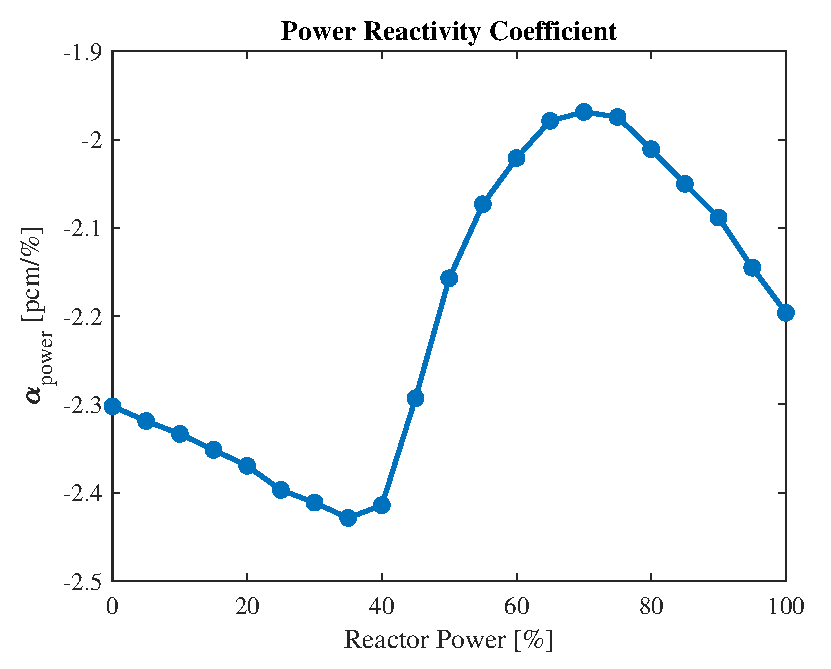
\includegraphics[width=0.5\textwidth]{alpha_power}}
    \hspace*{\fill}
    \subfloat[Thermal Expansion Reactivity Coefficient.]{
      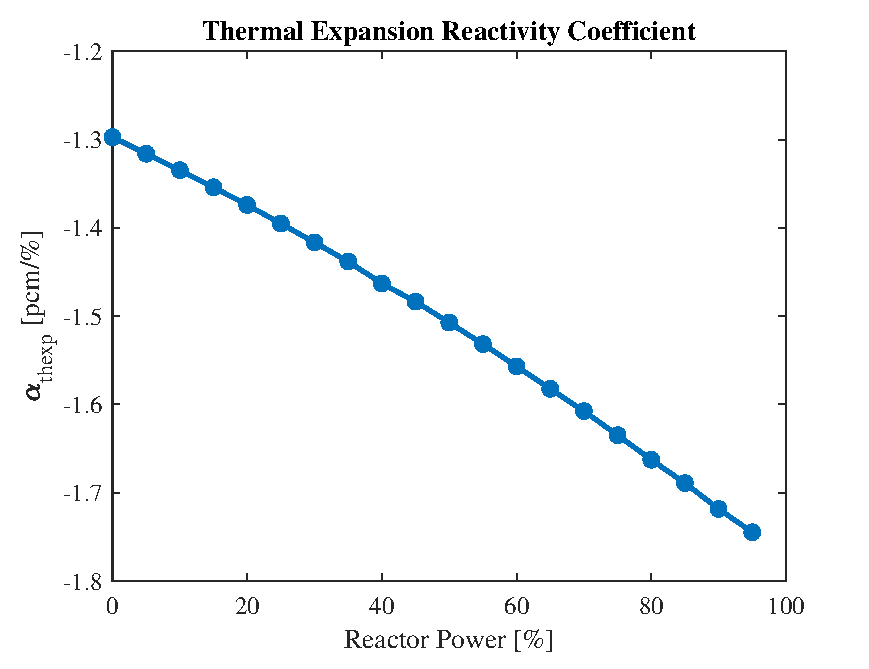
\includegraphics[width=0.5\textwidth]{alpha_thexp}}
    \vspace{\baselineskip}
    \subfloat[Doppler Reactivity Coefficient.]{
      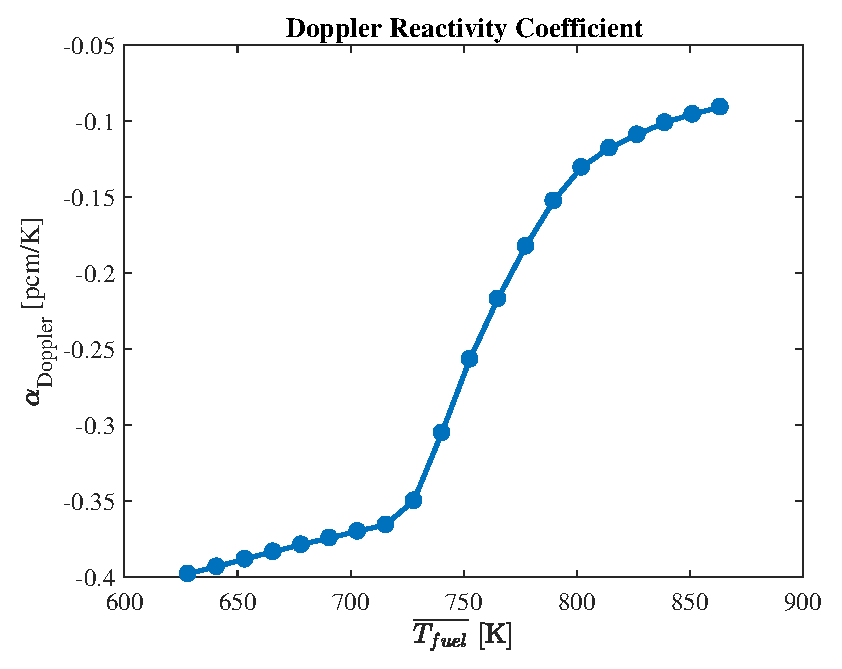
\includegraphics[width=0.5\textwidth]{alpha_fuel}}
    \hspace*{\fill}
    \subfloat[Coolant Temperature Reactivity Coefficient.]{
      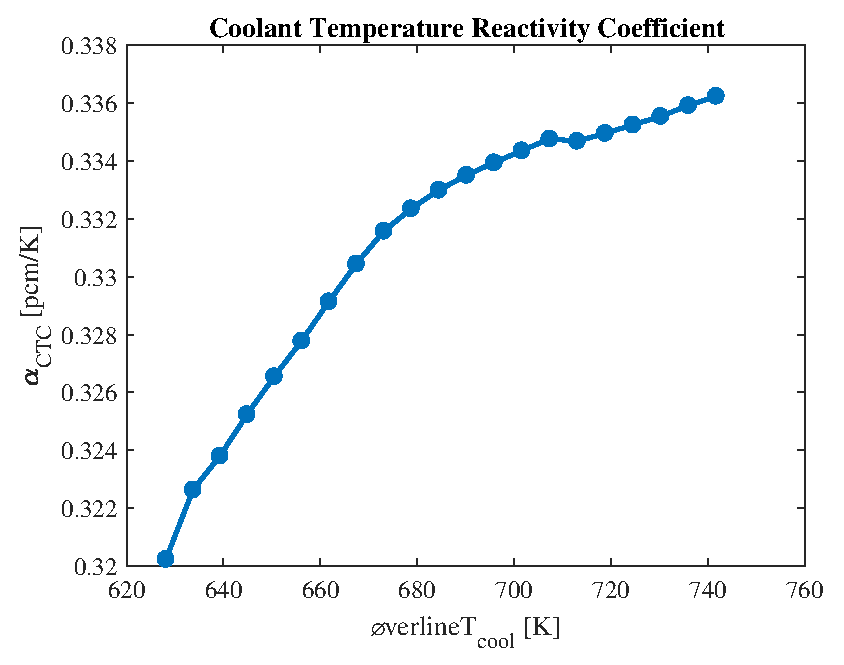
\includegraphics[width=0.5\textwidth]{alpha_cool}}
  \end{figure}

